\chapter{扩散}
    \section{扩散的微观机制}
        扩散的微观机制有四种,分别是\textbf{间隙扩散}\index{间隙扩散}、\textbf{环形扩散}\index{环形扩散}、\textbf{空位扩散}\index{空位扩散}、\textbf{挤列扩散}\index{挤列扩散}
        \subsection{间隙扩散}
            目前对于间隙扩散根据间隙原子尺寸分为两种情况考虑,可以有两种机制,分别是直接间隙机制和推填机制。

            对于尺寸较小的间隙原子,从一个间隙位置跳到相邻的空着的间隙位置,
            称为\textbf{直接间隙机制}\index{间隙扩散!直接间隙机制}。

            如果间隙原子尺寸较大,很难从一个间隙位置跳到另一个间隙位置,因为跳跃会造成很大的瞬时畸变能。
            因此提出另一种可能的扩散方式:位于间隙位置的原子把它位于最近邻的正常点阵
            位置的原子推入间隙位置,而自己占据该位置,这个机制称为\textbf{推填机制}\index{间隙扩散!推填机制},
            也称为\textbf{间接间隙机制}\index{间隙扩散!间接间隙机制}。
        \subsection{环行扩散}
            \textbf{环行扩散}\index{环行扩散}分为两种,分别是\textbf{直接交换}\index{环形扩散!直接交换}和\textbf{循环交换}\index{环形扩散!循环交换},
            具体过程如\autoref{环行扩散的两种机制}所示。
            \begin{figure}[ht]
                \centering
                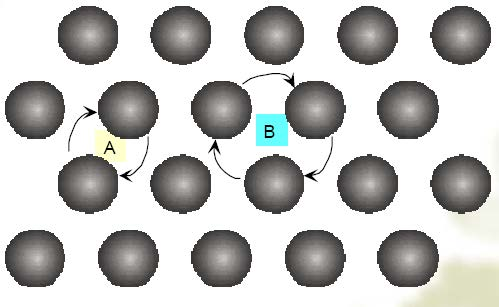
\includegraphics[width=0.5\textwidth]{fig/ring_diffusion.jpg}
                \caption{环行扩散的两种机制,其中A为直接交换,B为循环交换。}
                \label{环行扩散的两种机制}
            \end{figure}
        \subsection{空位扩散}
            \textbf{空位扩散}\index{空位扩散}对于晶体中存在的空位,空位周围的原子都是向空位进行扩散,
            扩散后形成新的空位。
        \subsection{挤列扩散}
            \textbf{挤列扩散}\index{挤列扩散}是在$n$个原子位置上挤进去一个原子,容纳了$n+1$个原子位置上挤进去一个原子,容纳了并作为
            一个整体沿挤列方向扩散。由于碱金属原子的压缩性较大,有可能形成这种组态。
    \section{Fick定律及其应用}
        \subsection{Fick第一定律}
            Fick 认为原子的扩散有具体的方向,应当从高浓度向低浓度扩散,以此得到了稳态下的Fick第一定律
            \begin{equation}
                J=-D\left( \frac{\partial c}{\partial x} \right)\label{Fick第一定律},
            \end{equation}
            上式称为\textbf{Fick第一定律}\index{Fick第一定律} ,其中 $J$为\textbf{扩散通量}\index{Fick第一定律!扩散通量},
            是某一时刻通过垂直于$x$轴的单位平面原子的通量;\textbf{扩散系数}\index{Fick第一定律!扩散系数}
            表示单位浓度梯度下的通量,上式表明,扩散方向与梯度方向相反。
            习惯上,\autoref{Fick第一定律}中各个量的单位为
            \begin{table}[ht]
                \centering
                \caption{Fick第一定律中各个物理量单位。}
                \label{Fick第一定律中各个物理量单位}
                \begin{tabular}{cc}
                    \toprule
                    物理量&单位\\
                    \midrule
                    $J$&\si{\g\per(\s\cdot\cm^2)}\\
                    $D$&\si{\cm^2\per\s}\\
                    $c$&\si{\g\per\cm^3}\\
                    $x$&\si{\cm}\\
                    \bottomrule
                \end{tabular}
            \end{table}
            
            对于三维空间,第一定律可以写作
            \begin{equation}
                J=-D\nabla c.
            \end{equation}
        \subsection{Fick第二定律}
            但是实际上,扩散通量$J$一般是不稳定的,伴随$x$变化,因此不同位置的浓度也会不同,
            对于$x_1$位置的$\dif x$厚度的体积元,单位时间的净通量为$J(x_1)-J(x_1+\dif x)$,
            其浓度改变速率为$\partial c/\partial t$,则有如下关系
            \begin{equation}
                \left( \frac{\partial c}{\partial t} \right)_{x_1}\dif x=J(x_1)-J(x_1+\dif x),
            \end{equation}
            当$\dif x\to0$时,有
            \begin{equation}
                J\left(x_{1}+\dif x\right)=J\left(x_{1}\right)+\left(\frac{\partial J}{\partial x}\right)_{x 1} \dif x
            \end{equation}
            所以有
            \begin{equation}
                \frac{\partial c}{\partial t}=-\frac{\partial J}{\partial x}=\frac{\partial}{\partial x}\left(D \frac{\partial c}{\partial x}\right),
            \end{equation}
            上式就是\textbf{Fick第二定律}\index{Fick第二定律}。
        
            一维情况下对于扩散系数$D$为常数的情况,Fick第二定律可以写作
            \begin{equation}
                D\left(\frac{\partial^{2} c}{\partial x^{2}}\right)=\frac{\partial c}{\partial t},
            \end{equation}
            对于扩散系数为变量的情况,Fick第二定律写作
            \begin{equation}
                \frac{\partial}{\partial x}\left[D\left(\frac{\partial c}{\partial x}\right)\right]=\frac{\partial c}{\partial t}.
            \end{equation}
            
            对于三维空间,在笛卡尔坐标系下,使用拉普拉斯算子,Fick第二定律可以写作
            \begin{equation}
                D\left(\frac{\partial^{2} c}{\partial x^{2}}+\frac{\partial^{2} c}{\partial y^{2}}+\frac{\partial^{2} c}{\partial z^{2}}\right)=\frac{\partial c}{\partial t}.
            \end{equation}

        \subsection{扩散方程的解}
            对于不同的类型,可以分为稳态扩散和非稳态扩散,其中\textbf{稳态扩散}\index{稳态扩散}
            是指空间各点的浓度不随时间发生变化,这种状态称为稳态扩散;\textbf{非稳态扩散}\index{非稳态扩散}是指
            空间中各点浓度随时间发生变化。
            \subsubsection{第一类稳态扩散}
                首先来看稳态扩散,假设扩散系数为常数,浓度不随时间发生变化。
                容器中间有金属薄板,薄板的一面保持高而恒定的浓度,另一面保
                持低而恒定的浓度,因此在金属板中存在浓度梯度。假设器壁不可渗透,
                经过一段时间,薄板中任一体积元,流入的和流出的通量相等,扩散达
                到稳定状态。
                
                此时的边界条件为$x=0$,$c=c_1$,$x=\Delta x$时,$c=c_0$,金属薄板的面积为$A$,
                总扩散通量为
                \begin{equation}
                    J_{\text{total}}=-AD\frac{\partial c}{\partial x},
                \end{equation}
                由于问题属于一维问题,可以将偏微分改为全微分
                \begin{equation}
                    J_{\text{total}}=-AD\frac{\dif c}{\dif x},
                \end{equation}
                两边同时乘以$\dif x$并在$0\to\dif x$范围内积分,有
                \begin{equation}
                    \int_{0}^{\Delta x}J_{\text{total}}\dif x=-\int_{c_{1}}^{c_{0}} A D \dif c
                \end{equation}
                得到
                \begin{equation}
                    J_{\text{total}}=\frac{AD(c_1-c_0)}{\Delta x}.
                \end{equation}

                这一类模型可以模拟钢铁真空脱气,假设金属表面溶解度与相接触的气体压力有关,对于
                双原子气体有
                \begin{equation}
                    c=S\sqrt{p},
                \end{equation}
                单位面积的扩散通量就可以写作
                \begin{equation}
                    J=\frac{D S\left(\sqrt{p_{1}}-\sqrt{p_{0}}\right)}{\Delta x}.
                \end{equation}
            \subsubsection{第二类稳态扩散}
                这类问题扩散是指空间各点的浓度不随时间发生变化,但是扩散系数$D$不是常数。
                有人利用这一特点模拟了碳在$\gamma$铁中的扩散过程并测量了扩散系数。

                将长度为$l$、半径为$r$的薄壁铁管在\SI{1000}{\celsius}下退火,管内
                是渗碳气氛,关外是脱碳气氛,当时间最够长时,壁管内各点的碳浓度不再随时间而变,
                也就是
                \begin{equation}
                    \frac{\partial c}{\partial t}=0.
                \end{equation}
                达到稳定状态后,设$t$时间内通过管壁的碳量为$q$,则单位时间通过
                的碳量$q/t$为常量。因而,单位时间流入或流出单位面积的通量为
                \begin{equation}
                    J=\frac{q}{2\pi lt},
                \end{equation}
                根据\autoref{Fick第一定律}可得
                \begin{equation}
                    \frac{q}{2\pi lt}=-D\frac{\dif c}{\dif r},
                \end{equation}
                解得
                \begin{equation}
                    q=-D\left( 2\pi lt \right)\frac{\dif c}{\dif \ln r},
                \end{equation}
                式中,$q$,$l$,$t$以及碳沿管壁的径向分布都可以测量,扩散系数$D$
                可以由$c$对$\ln r$的斜率确定。

            \subsubsection{第一类非稳态扩散}
                这种情况是空间各点的浓度随时间发生变化,但是$D$为常数的情况,
                此时的Fick第二定律可以写作
                \begin{equation}
                    \frac{\partial c}{\partial t}=D \frac{\partial^{2} c}{\partial x^{2}}.
                \end{equation}
                这一公式可以解决两种模型,分别为\textbf{瞬时平面源}\index{瞬时平面源}和\textbf{一维半无限模型}\index{一维半无限模型}(也称为叠加法)。

                对于瞬时平面源模型,假设两块足够长的相同纯金属,其中
                一块端面上涂上同位素(作为扩散面源),对接起来组成扩散偶,假设扩散系数为常数
                Fick第二定律的解的形式为
                \begin{equation}
                    c=\frac{A}{\sqrt{t}} \exp \left(-\frac{x^{2}}{4 D t}\right),
                \end{equation}
                式中$A$为待定系数。由于扩散总量一定,为$M$,也就是
                \begin{equation}
                    \int_{-\infty}^{\infty} c(x, t) \mathrm{d} x=M,
                \end{equation}
                可以解得
                \begin{equation}
                    c(x, t)=\frac{M}{2 \sqrt{\pi D t}} e^{-\frac{x^{2}}{4 D t}}
                \end{equation}

                对于另一种模型,则是假设一块无限长的金属,$x<0$为扩散源,$x>0$为被扩散物质。
                首先求解单位体积元扩散对$x>0$的某一点的影响,该点的总浓度就是所有体积元作用的总和。
                求解过程相对复杂,这里直接给出结果
                \begin{equation}
                    c(x, t)=\frac{c_{0}}{2}\left[1-\operatorname{erf}\left(\frac{x}{2 \sqrt{D t}}\right)\right]
                \end{equation}
                其中$\operatorname{erf}$为误差函数,其有数值表可以查阅。
                假设初始浓度为$c=c_0$,扩散时,表面浓度恒定为$c=c_s$,则上式可以写作
                \begin{equation}
                    c(x,t)=c_0+(c_s-c_0)\left[ 1-\operatorname{erf}\left( \frac{x}{2\sqrt{Dt}} \right) \right],
                \end{equation}
                这一公式适用于工业上工件的渗碳过程。

                这里还有一个概念性的常用关系式,当某一处的浓度满足
                \begin{equation}
                    \frac{c-c_{0}}{c_{s}-c_{0}}=\frac{1}{2},
                \end{equation}
                该处对应的位置为
                \begin{equation}
                    x_{\frac{1}{2}}=\sqrt{Dt},
                \end{equation}
                这一位置的$x$称为\textbf{半浓度深度}\index{Fick第二定律!半浓度深度},记作$x_{1/2}$,
                对与任意时间都成立。

                对于温度改变的系统,测量此时的\textbf{扩散系数}\index{Fick第二定律!扩散系数} ,可以发现其与温度有明显的关系,一般可以写作
                \begin{equation}
                    D=D_0\exp\left( -\frac{Q}{RT} \right),
                \end{equation}
                上式称为\textbf{Arrhenius关系}\index{Fick第二定律!扩散系数!Arrhenius关系},其中$Q$为
                扩散激活能,式中$Q$、$D_0$与温度无关,与成分、结构有关。
            \subsubsection{第二类非稳态扩散}
                这一类问题研究$D$随浓度变化的全无限长的一维扩散。如果将铜和
                黄铜对接起来,组成浓度差很大的扩散偶,则D因浓度而变。\ce{Zn}的浓度初始分布为
                $x>0$,$c=c_0$,$x<0$,$x=0$,对此解偏微分方程
                \begin{equation}
                    \frac{\partial c}{\partial t}=\frac{\partial }{\partial x}\left( D\frac{\partial c}{\partial x} \right),
                \end{equation}
                某处浓度为$c_1$,求得其扩散系数
                \begin{equation}
                    D_{c_1}=-\frac{1}{2t}\left.\frac{\dif x}{\dif c}\right\vert_{c=c_1}\cdot\int_{0}^{c_1}x\dif c\label{扩散系数随浓度变化关系},
                \end{equation}
                式中$\frac{\dif x}{\dif c}\vert_{c=c_1}$为$c-x$曲线上$c=c_1$处的斜率,$\int_{0}^{c_1}x\dif c$为积分面积。
                这样可以解决扩散系数问题,但是$\int_{0}^{c_1}x\dif c$中,$x$的原点不一定是是原始的焊接面,
                因此在求解扩散系数时必须先确定\textbf{Matano面}\index{Matano面} ,也就是在这个面两侧的$c-x$曲线积分面积相等,
                也就是$\int_{0}^{c_1}x\dif c=0$,为了区分Matano面和原始焊接面,后者记作$x'=0$。因此在
                实际中求解某处的扩散系数一般要四步
                \begin{itemize}
                    \item[1] 在一定温度$T$下,是扩散偶退火一定时间$t$,分析浓度$c$,作出$c-x$曲线;
                    \item[2] 使两边积分面积相等,确定Matano面;
                    \item[3] 求$c_1$处的切线斜率和积分面积$\int_{0}^{c_1}x\dif c$;
                    \item[4] 代入\autoref{扩散系数随浓度变化关系},求出$D_{c_1}$。
                \end{itemize}

                关于Matano面,有以下两点结论:
                \begin{itemize}
                    \item[1] 扩散过程中,体积保持不变时,焊接面和Matano面一致;
                    \item[2] Matano面分割物质的流动体积,使一边流出的物质量等于另一边流入的量。
                \end{itemize}
            \subsubsection{均匀化速率问题}
                在实际中,经常遇到不均匀合金的均匀化问题,如奥氏体化时第
                二相的溶解速度问题,铸态合金的均匀化问题\index{均匀化问题}等。

                在不均匀合金中,如果浓度沿某一方向呈周期性变化,则合金的初始浓度分布可以用下式来表示
                \begin{equation}
                    c(x)=c_0+c_m\cos\left( \frac{\pi x}{l} \right).
                \end{equation}
                对于这一类问题的Fick方程的解为
                \begin{equation}
                    c(x, t)=c_{0}+c_{m} \cos \left(\frac{\pi x}{l}\right) \exp \left(-\frac{t}{\tau}\right),
                \end{equation}
                其中$\tau=\frac{l^2}{\pi^2D}$称为\textbf{弛豫时间}\index{均匀后问题!弛豫时间}。减少弛豫时间
                可以加速体系均匀化,可以采用升高温度或减少长度的方法,由于温度的改变导致扩散系数的改变对结果的影响
                不大,因此主要采用减少长度的方法,因此需要快冷、锻打。
    
    \section{原子迁移和扩散系数}
        \subsection{扩散系数的统计性}   
            扩散的宏观现象是由大量原子的无数次随机行走造成的。只有用统计概念才能计算扩散系数。
            之前的Fick定律认为体系的扩散方向为顺浓度方向,然而实际中还存在着"上坡"扩散这样的
            例外,这只能从能量角度来解释,也就是说,扩散的真正驱动力为化学位梯度而不是浓度梯度。

            对于两个临近晶面,原子面密度分别为$n_1$和$n_2$,假设每次迁移的距离都是$\alpha$,
            一个原子单位时间内迁移$\Gamma$次,则$\delta t$时间内从面1跳出的原子数为
            $n_1\Gamma\delta t$。如果迁移方向是随机的,对于三维问题,则从晶面1迁移
            到晶面2的概率就是$1/6$,在$\delta t$时间内从1跳到2的原子数为$\frac{1}{6}n_1\Gamma\delta t$,
            同理从2跳到1的原子数为$\frac{1}{6}n_2\Gamma\delta t$,则面1到面2的净通量为
            \begin{equation}
                J=\frac{1}{6}(n_1-n_2)\Gamma\label{迁移通量与面密度关系},
            \end{equation}
            面密度和浓度的关系为
            \begin{equation}
                \frac{n}{\alpha}=c,
            \end{equation}
            因此净通量写作
            \begin{equation}
                J=\frac{1}{6}\alpha\left( c_1-c_2 \right)\Gamma.
            \end{equation}
            由于
            \begin{equation}
                \frac{\partial c}{\partial x}=\frac{c_2-c_1}{\alpha},
            \end{equation}
            得到
            \begin{equation}
                J=-\frac{1}{6}\alpha^2\Gamma\frac{\partial c}{\partial x},
            \end{equation}
            与Fick第一定律比较得到
            \begin{equation}
                D=\frac{1}{6}\alpha^2\Gamma\label{扩散系数与迁移率和迁移距离关系},
            \end{equation}
            可知扩散系数正比于迁移率和迁移距离的平方。
            从以上的讨论也可以看出,决定迁移净通量的是不同原子面之间的面密度而不是浓度梯度。

            对于fcc和hcp金属来说,在熔点附近的迁移率为\SI{1e8}{\s^{-1}},但是实际上原子热振动频率为
            \numrange{1e12}{1e13},原子在平衡位置振动\numrange{1e4}{1e5}次才会成功跳离一次。

            一般来说,迁移距离随温度的变化不大,这只和点阵类型和点阵常数有关系,扩散速率
            与温度的关系主要取决于迁移率$\Gamma$,假设
            \begin{equation}
                \Gamma=Zp_v\omega,
            \end{equation}
            其中$Z$为配位数,$p_v$为近邻是空位置的几率,$\omega$原子迁入空位的频率,
            代入\autoref{扩散系数与迁移率和迁移距离关系}可得
            \begin{equation}
                D=\frac{1}{6}\alpha^2Zp_v\omega.
            \end{equation}

    \section{扩散系数与浓度}
        \subsection{Kirkendall效应}
            这里不再叙述\href{http://www.phase-trans.msm.cam.ac.uk/kirkendall.html}{Kirkendall效应}\index{Kirkendall效应}的实验过程,
            直接说明结论,对于由A、B两种原子组成的体系,$D_A>D_B$引起的\textbf{标记面}\index{Kirkendall效应!标记面}的移动称为Kirkendall效应。
            其不可能使用原子交换机制进行迁移,因为如果扩散使用原子交换进行,对于任意平面来说,净通量
            都为零。
        \subsection{Darken公式}
            A、B原子的百分比分别为$N_1=c_1/c$、$N_2=c_2/c$,扩散系数分别为$D_1$、$D_2$,
            标记面移动速度为$V$,得出\textbf{Darken公式}\index{Darken公式}
            \begin{align}
                \widetilde{D}&=N_{2} D_{1}+N_{1} D_{2},\\
                v&=\left(D_{2}-D_{1}\right) \frac{\partial N_{2}}{\partial x},\\
                v&=\left(D_{1}-D_{2}\right) \frac{\partial N_{1}}{\partial x}
            \end{align}
            以上三式合称Darken公式。在一定浓度下测得化学扩散系数$\widetilde{D}$、标记面移动速度$V$
            和浓度梯度,就可以确定该浓度下的\textbf{偏扩散系数}\index{偏扩散系数}$D_1$、$D_2$,它们是浓度梯度下
            组元的扩散系数,称$\widetilde{D}$为\textbf{化学扩散系数}\index{Darken公式!化学扩散系数}或互扩散系数。

        \subsection{总结}
            目前已经接触了三个平面,分别是原始焊接平面($S_0$)\index{原始焊接平面},Matano面($S_M$)\index{Matano面}
            和标记面($S_I$)\index{Kirkendall效应!标记面},这里总结在不同条件下它们的相对位置的变化,
            从而建立扩散过程中物质流动的明确图像。
            \begin{itemize}
                \item[1] 当$\frac{\dif c}{\dif t}=0$,且$D_1=D_2$时,$V=0$,所以$S_0=S_I$,而且$J_1=-J_2$,所以$S_0=S_M$,三个面重合;
                \item[2] 当$\frac{\dif c}{\dif t}=0$,$D_1\neq D_2$时,$J_1\neq J_2$,$S_I\neq S_0$,但是$S_0=S_m$;
                \item[3] 当$\frac{\dif c}{\dif t}\neq0$,$D_1=D_2$时,$S_0\neq S_M$,但是$S_I=S_M$;
                \item[4] 当$\frac{\dif c}{\dif t}\neq0$,且$D_1\neq D_2$时,三个面均不相等。
            \end{itemize}
            总结一下,偏扩散系数相等时,标记面和Matano面相等;空间中浓度不随时间发生变化时,焊接面和Matano面相等。

            关于Fick定律和Kirkendall效应有以下几点说明
            \begin{itemize}
                \item 每一种原子都有其自身的本征扩散系数;
                \item 原子成功跃迁的几率依赖于结合键被拆断的难易程度,因此与金属的熔点有关;
                \item 扩散的全部结论,或者说Fick定律中的扩散系数是不同种类原子本征扩散的综合作用的函数,即Darken公式;
                \item 由于不同的本征扩散系数,Fick定律中的扩散系数是成分的函数。Matano面的构架是评价扩散系数对浓度的依赖性的一个方法;
                \item 由于本征扩散系数不同,在扩散偶中存在空位的净通量。当两边的空位各自重新排列趋向平衡时,两边的合金就改变了相对体积。这引起了界面移动,即Kirkendall效应;
                \item 跃迁频率和扩散系数之间的简单关系对自扩散是有效的,对稀固溶体是很好的近似。
            \end{itemize}
    \section{反应扩散}
        在许多合金状态图中有中间相,因而扩散过程中也可能出现中间相,这种扩散即为\textbf{多相扩散}\index{多相扩散}。

        多相扩散包括两个过程,分别是扩散过程和界面上达到一定的浓度发生化学反应,从而形成新相的过程。

        通过扩散使固溶体内的溶质组元超过固溶度限而不断形成新相的过程就是\textbf{反应扩散}\index{反应扩散}由反应扩散所产生的新相,可以是新的固
        溶体,也可以是化合物。

        反应扩散的特点是在相界面处产生浓度突变,突变的浓度正好对应于相的极限溶解度。
        根据相律关系,自由度$F$、族元数$C$和相数$P$关系为
        \begin{equation}
            F=C-P+2,
        \end{equation}
        但是在扩散过程中,温度和压力一定,因此应当去掉两个自由度,此时$F=C-P$,
        \begin{itemize}
            \item 单相情况下,$P=1$,$C=2$,于是$F=2-1=1$,说明该相的浓度是可以改变的,因此在扩散过程中可以有浓度梯度,即扩散过程可以发生;
            \item 在双相去,$F=2-2=0$,意味着在双相区中,各相的浓度不能改变,它与状态图中的极限溶解度相对应,说明在两相区中不存在浓度梯度。
        \end{itemize}
        
        \subsection{新相长大的动力学}
            由纯金属A、B组成的扩散偶,在各自的\textbf{边际固溶体}\index{一次固溶体!边际固溶体}中存在有
            极限溶解度。经过时间$t$后的浓度分布曲线为